\documentclass{article}
\usepackage{enumitem}
\usepackage{array}
\usepackage{subcaption}
\usepackage{graphicx}
\usepackage{subcaption}

\usepackage{color}
\usepackage[top=1in,bottom=1in,left=1.2in,right=1.2in]{geometry}
\usepackage{hyperref}
\usepackage[small]{titlesec}
\usepackage{booktabs}
\usepackage{colm2024_conference}
\usepackage{graphicx}
\usepackage[dvipsnames]{xcolor}
\usepackage{rotating}
\usepackage{pdflscape}
\usepackage{amsmath}

\newcommand{\todo}[1]{\textcolor{red}{\textbf{TODO:} #1}}

% Commenting
\newcommand{\eat}[1]{\ignorespaces}
%% Comment this line and uncomment the next to hide all comments
\newcommand{\xxcomment}[4]{\textcolor{#1}{[$^{\textsc{#2}}_{\textsc{#3}}$ #4]}}
\newcommand{\ta}[1]{\xxcomment{blue}{T}{A}{#1}}

\DeclareMathOperator{\softplus}{softplus}

\title{CS5787: Exercises 3 \\ \begin{small}\url{https://github.com/mitkrieg/dl-assignment-3}\end{small}}
\author{Mitchell Krieger \\ mak483@cornell.edu}

\date{}

\colmfinalcopy
\begin{document}
\maketitle

\section{Theory: Question 1 [40 pts]}

\begin{enumerate}[label=\alph*)]
    \item $\theta \neq 0$
        \begin{itemize}
            \item KL Divergence: \\ When $\theta = 0$ there is no overlap between P and Q. This means that whenever P is greater than zero, Q is zero. Applying this to the 
            KL formula at $x=0$ and assume that we can represent x as the Dirac delta function $\delta(x)$, and $u(y)$ is the uniform distribution over [0,1].
            \begin{equation}
                \begin{aligned}
                    D_{KL}(P||Q) &= \int_{x=-\infty}^{\infty} \int_{y=-\infty}^{\infty} P(x,y)\log \frac{P(x,y)}{Q(x,y)}dydx
                    \\ &= \int_{x=-\infty}^{\infty} \int_{y=-\infty}^{\infty} \delta(x)\cdot u(y)\log \frac{\delta(x)\cdot u(y)}{\delta(x-\theta)\cdot u(y)}dydx
                    \\ &= \int_{x=-\infty}^{\infty} \delta(x)  \int_{y=0}^{1} \log(\frac{\delta(x)\cdot 1}{\delta(x-\theta)\cdot 1}) dx
                \end{aligned}
            \end{equation}
            Since, $\delta(x)$ is zero everywhere except $x=0$
            \begin{equation}
                \begin{aligned}
                    D_{KL}(P||Q) &= \int_{y=0}^{1} \log(\frac{\delta(0)}{\delta(-\theta)}) dy
                    \\ &=  \frac{\delta(0)}{0} = \infty
                \end{aligned}
            \end{equation}
            We can see from the above that because the logarithm in the equation is undefined, we get a value for KL Divergence that tends to $\infty$.\\
            \item JS Divergence: \\ The JS Divergence considers the KL Divergence between each distribution and the average of the two distributions.
            The average distribution $\frac{P+Q}{2}$ will split the distribution to be half at $x = 0$ and half at $x = \theta$. Therefore, The KL Divergence between
            P and the average will be:
            \begin{equation}
                \begin{aligned}
                    D_{KL}(P||\frac{P+Q}{2}) &= \int_{x=-\infty}^{\infty} \int_{y=-\infty}^{\infty} P(x,y)\log \frac{P(x,y)}{\frac{1}{2}P(x,y)+\frac{1}{2}Q(x,y)}dydx
                    \\ &= \int_{x=-\infty}^{\infty} \delta(x)  \int_{y=0}^{1} \log(\frac{\delta(x)\cdot u(y)}{\frac{1}{2}\delta(x)\cdot u(y)+\frac{1}{2}\delta(x-\theta)\cdot u(y)})
                \end{aligned}
            \end{equation}
            Since, $\delta(x)$ is zero everywhere except $x=0$, and $\delta(x-\theta) = 0$ at $x=0$
            \begin{equation}
                \begin{aligned}
                    D_{KL}(P||\frac{P+Q}{2}) &= \int_{y=0}^{1} \log(\frac{\delta(0))\cdot u(y)}{\frac{1}{2}\delta(0)\cdot u(y)+\frac{1}{2}\cdot0\cdot u(y)})
                    \\  &=  \log(\frac{1}{\frac{1}{2}}) 
                    \\  &= \log(2)
                \end{aligned}
            \end{equation}

            $D_{KL}(Q||\frac{P+Q}{2})$ will give the same result. So applying the JS Divergence formula:
            \begin{equation}
                \begin{aligned}
                    D_{JS}(P||Q) = \frac{1}{2} \cdot \log(2) + \frac{1}{2} \cdot \log(2) = \log(2)
                \end{aligned}
            \end{equation}
            \\
            \item Wasserstein Distance: \\ The Wasserstein Distance is $\theta$ because both distributions have the same uniform distribution between [0,1] for $y$. 
            Because they are identical except for the x-value of P is 0 and the x-value of Q is $\theta$, the cost of moving P to Q would be $\theta$.
        \end{itemize}  
    \item $\theta = 0$
        \begin{itemize}
            \item KL Divergence: \\ Zero because the distributions are the same
            \begin{equation}
                \begin{aligned}
                    D_{KL}(P||Q) &= \int_{-\infty}^{\infty} \int_{-\infty}^{\infty} P(x)\log \frac{P(x,y)}{P(x,y)}dydx\\
                    &= \int_{-\infty}^{\infty} \int_{-\infty}^{\infty} P(x,y)\log1 dydx\\
                    &= \int_{-\infty}^{\infty} \int_{-\infty}^{\infty} 0\cdot P(x,y)  dydx\\
                    &= 0
                \end{aligned}
            \end{equation}
            \item JS Divergence: \\ $\frac{P+Q}{2} = P = Q$ because both distributions are uniform between [0,1] for $y$ and centered at $x = 0$. So the JS Divergence is zero because the distributions are the same
            \begin{equation}
                \begin{aligned}
                    D_{JS}(P||Q) &= \frac{1}{2}D_{KL}(P||\frac{P+Q}{2}) + \frac{1}{2}D_{KL}(Q||\frac{P+Q}{2}) \\
                                 &= \frac{1}{2} \cdot 0 + \frac{1}{2} \cdot 0 = 0
                \end{aligned}
            \end{equation}
            \item Wasserstein Distance: Zero because both distributions are uniform between [0,1] for $y$ and centered at $x = 0$. So there is no cost to transform P into Q.
    
    \end{itemize}  
    \item The advantage of the Wasserstein Distance is that it is both interpretable and stable when compared to KL and JS Divergence. When $\theta \neq 0$,
    KL is infinite and JS is $\log2$, where as Wasserstein is $\theta$. In this context, $\theta$ is a much clearer measure of the distances between the two 
    distribution because it is simply the distance between the x-values of the distributions. In addition, both KL and JS have discontinuous jumps from when 
    they overlap to when then don't, KL becomes infinite and JS although still finite jumps from 0 to $\log2$. Wasserstein distance on the other hand, increases linearly as 
    $\theta$ grows. These are big advantages because it would make the gradient in training a model more stable because it is continuous and not super sensitive to small changes (from not overlapping to overlapping).

\end{enumerate}


\section{Theory: Question 2 [10 pts]}

LSTMs will process inputs sequentially. So at each time step, the LSTM will have to multiply the input by the hidden state, the previous hidden state by the current hidden state,
and other smaller operations like the activation functions for the gates and addition for adding bias and cell state updates. The dominant operation here is the multiplication of the 
hidden states. This operation has a time complexity of $O(d^2)$ where $d$ is the dimension of the hidden state. Because we do this at every time step t for all $N$, the total complexity is $O(d^2N)$.
However, the size of the hidden state is a constant value, and not a function of the size of the input, so the total time complexity is linear $O(N)$.

Transformers on the other hand use self-attention, which requires every value of the input to be compared to all other values in the input. This is an $O(N^2)$ operation. The other components
of transformers, such as the feed forward network, encoder/decoder and positional encoding are all generally $O(N)$, so they get dominated by the self-attention mechanism's computational complexity.
So the total time complexity is quadratic at $O(N^2)$

\section{Practical: Question 3 [5 pts]}

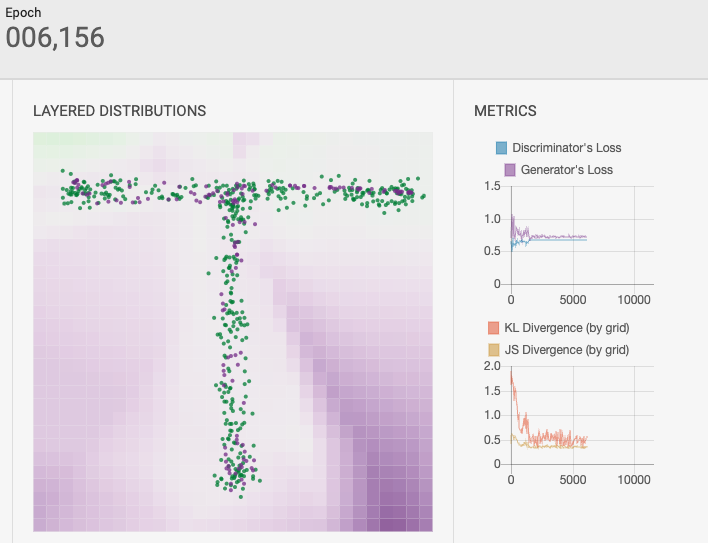
\includegraphics[scale=.5]{../src/gan_lab.png}

\section{Practical: Question 4 [20 pts]}

The goal for this problem was to implement the M1 architecture described in "Semi-supervised Learning with Deep Generative Models" (Kingsma et al.) for the Fashion MNIST dataset.
M1 attempts to build a generative model that can create images in the likeness of the the data using a Variational autoencoder (VAE) with an SVM head. This model was trained using a 
semi-supervised method. The encoder in the VAE aims to predict the mean and variance of the distribution over the latent variable $z$. However, because of the random nature of $z$,
we are unable to take the derivative of it which means it can't be used in back propagation. To address this, the reparameterization trick is used, where instead of directly sampling from this distribution
we sample from the standard gaussian distribution and then shift it by the mean and variance predicted by the encoder. Then the decoder uses this sample to reconstruct an image. 

In addition, an SVM with a radial basis function kernel is trained as a head for this model to classify the generated images using the latent representations created by the encoder as input. Two SVMs were trained for each model using different regularization parameters,
and the one with the better accuracy was chosen.

Four VAE models were trained each with an increasing number of labeled samples 100, 600, 1000 and 3000, and the results are described in the table below:

\begin{table}[h]
    \centering
    \begin{tabular}{|c|c|}
    \hline
    N    & SVM Head Test Set Accuracy \\
    \hline
    100  & 0.5957                     \\
    \hline
    600  & 0.7015                     \\
    \hline
    1000 & 0.7093                     \\
    \hline
    6000 & 0.7291 \\
    \hline               
    \end{tabular}
\end{table}

\newpage
An example of the generated output and the SVM prediction is below:

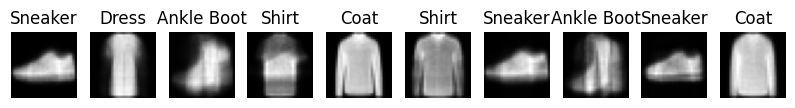
\includegraphics[scale=0.7]{../src/svm_predict.png}

\section{Practical: Question 5 [25 pts]}

The goal of was to also build a generative model that can create images in the likeness of the Fashion MNIST dataset but this time using 3 GAN methods (DCGAN, WGAN with clipping, WGAN-GP) over 2 different architectures.
Both architectures used have a discriminator/critic that consists of 4 convolutional layers with a kernel size of 4, stride of 2 and padding of 1 (except for the final layer has 
zero padding), followed by a fully connected layer. The generator has these same layers in reverse order. The main difference between the two architectures is the use of normalization
and choice of activation function. In architecture A, Leaky ReLU was used with a negative slope of 0.2 as an activation function. In addition, BatchNorm (or LayerNorm in WGAN-GP) was used for normalization.
Architecture B on the other hand, uses an adjusted softplus, $\frac{\softplus(2x+2)}{2}$ and has no normalization. \\
\\

\begin{figure}[ht]
    \caption{Real Pullovers compared with Generated Pullovers}
    \centering
    % Left side: Two side-by-side images
    \resizebox{0.6\textwidth}{!}{
    \begin{minipage}[t]{0.45\textwidth}
        \vfill
        \centering
        \begin{minipage}[b]{0.45\textwidth}
            \centering
            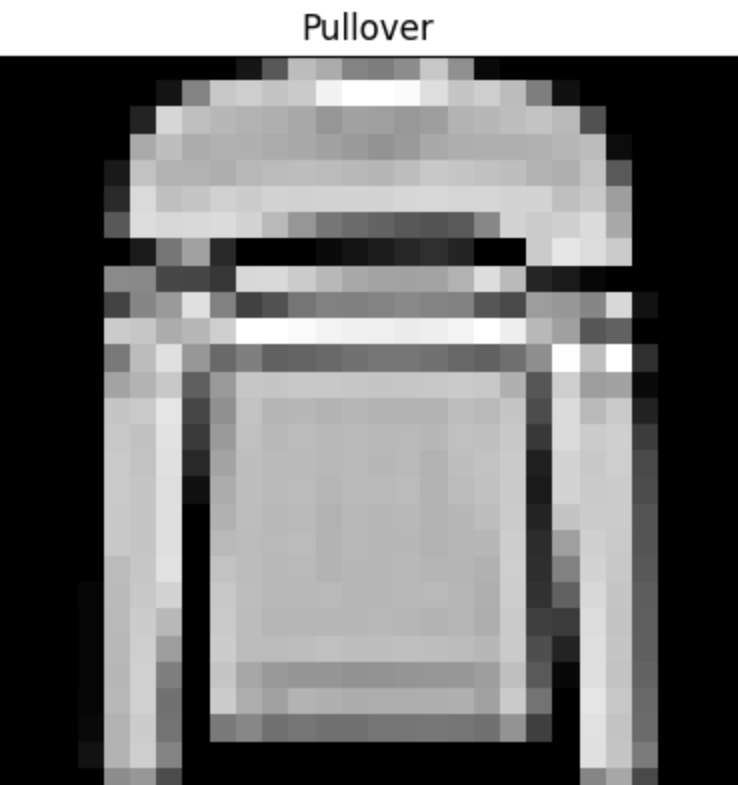
\includegraphics[width=\textwidth]{../src/real_pullover1.png}
            % \caption{Real Sample 1}
            % \label{fig:image4}
        \end{minipage}
        \hfill
        \begin{minipage}[b]{0.45\textwidth}
            \centering
            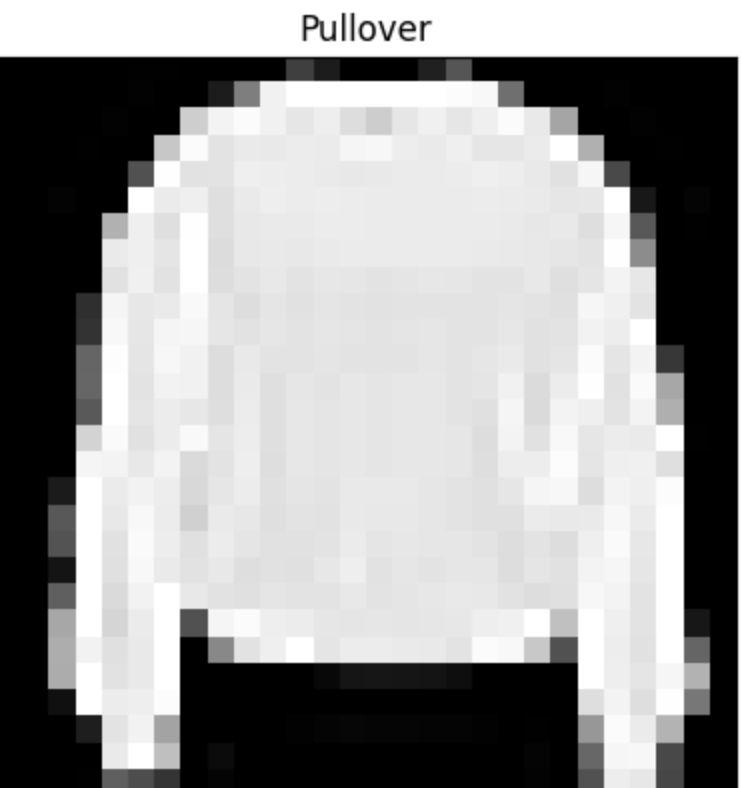
\includegraphics[width=\textwidth]{../src/real_pullover2.png}
            % \label{fig:image5}
        \end{minipage}
        \vfill
    \end{minipage}
    \hfill
    % Right side: Three stacked images
    \begin{minipage}[t]{0.45\textwidth}
        \centering
        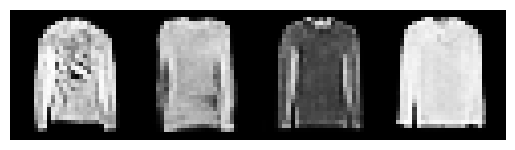
\includegraphics[width=\textwidth]{../src/dc_pullover.png}
        \caption{DCGAN}
        \label{fig:image1}
        \vspace{0.1cm} % Space between the images

        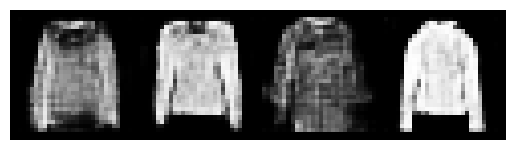
\includegraphics[width=\textwidth]{../src/wgan_pullover.png}
        \caption{WGAN with Weight Clipping}
        \label{fig:image2}
        \vspace{0.1cm} % Space between the images

        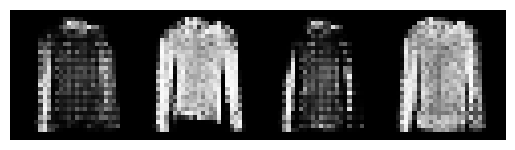
\includegraphics[width=\textwidth]{../src/gp_pullover.png}
        \caption{WGAN-GP}
        \label{fig:image3}
    \end{minipage}
    }
\end{figure}


\begin{figure}[ht]
    \caption{Real Ankle Boot compared with Generated Ankle Boot}
    \centering
    % Left side: Two side-by-side images
    \resizebox{0.6\textwidth}{!}{
    \begin{minipage}[t]{0.45\textwidth}
        \vfill
        \centering
        \begin{minipage}[b]{0.45\textwidth}
            \centering
            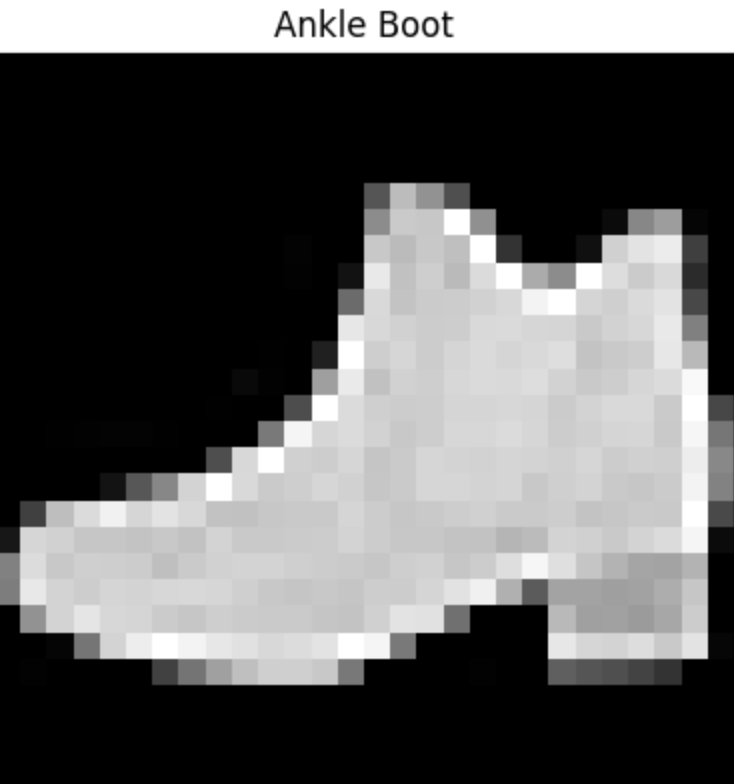
\includegraphics[width=\textwidth]{../src/real_boot1.png}
            \label{fig:image4}
        \end{minipage}
        \hfill
        \begin{minipage}[b]{0.45\textwidth}
            \centering
            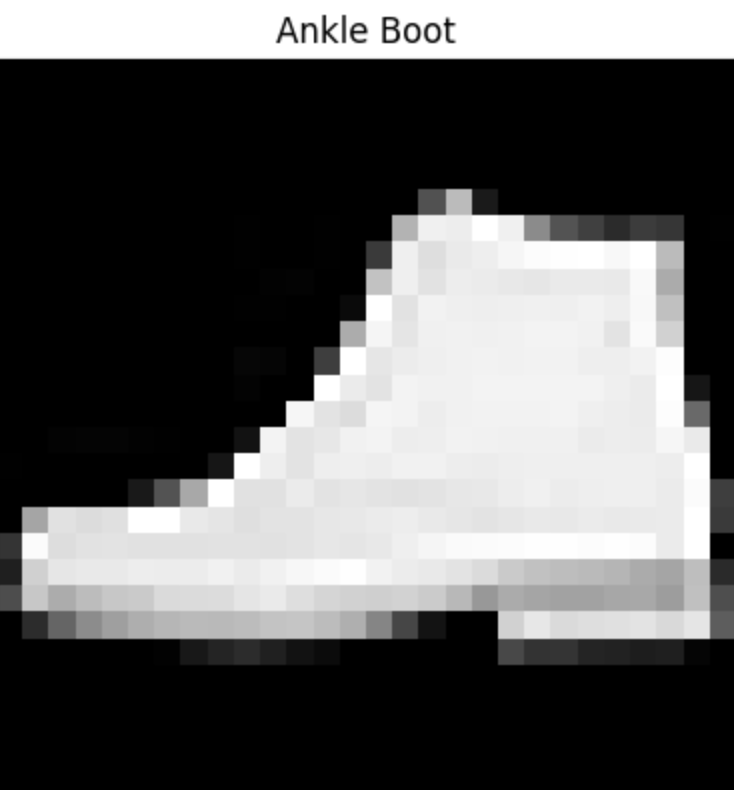
\includegraphics[width=\textwidth]{../src/real_boot2.png}
            \label{fig:image5}
        \end{minipage}
        \vfill
    \end{minipage}
    \hfill
    % Right side: Three stacked images
    \begin{minipage}[t]{0.45\textwidth}
        \centering
        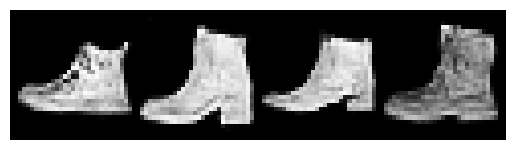
\includegraphics[width=\textwidth]{../src/dc_boot.png}
        \caption{DCGAN}
        \label{fig:image1}

        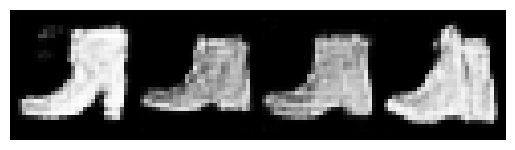
\includegraphics[width=\textwidth]{../src/wgan_boot.png}
        \caption{WGAN with Weight Clipping}
        \label{fig:image2}

        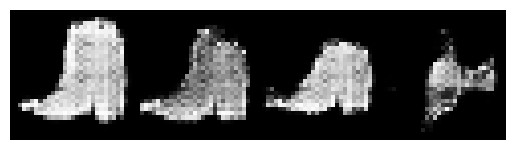
\includegraphics[width=\textwidth]{../src/gp_boot.png}
        \caption{WGAN-GP}
        \label{fig:image3}
    \end{minipage}  
    }
\end{figure}

Architecture A had consistently better visual results after training for 10 epochs. The figures above display real samples for two classes (ankle boot and pullover) on the left compared with generated samples on the right for architecture A with each
GAN method. All three models, generate images that are in the likeness of Fashion MNIST.  

Loss for each model's generator and discriminator/critic has been plotted below as well.
For all three models, we can see that the loss curves for architecture A converges much better than B (there was an order of magnitude difference between A
and B loss for WGAN and WGAN-GP so zoomed in plots are provided on the following page). WGAN-GP's loss oscillates more frequently and has larger swings in later epochs suggesting
that we may have been able to achieve the same results in less epochs. To train these models, it was easier to find convergence on WGAN and WGAN-GP than on DCGAN. For DCGAN,
training was run 5 or 6 times before finding convergence. Where as with WGAN and WGAN-GP there was only 1 failed convergence and the rest converged (even if it was to a poor result).

\begin{figure}[ht]
    \centering
    % First row
    \caption{Loss Curves}
    \begin{minipage}[b]{0.45\textwidth}
        \centering
        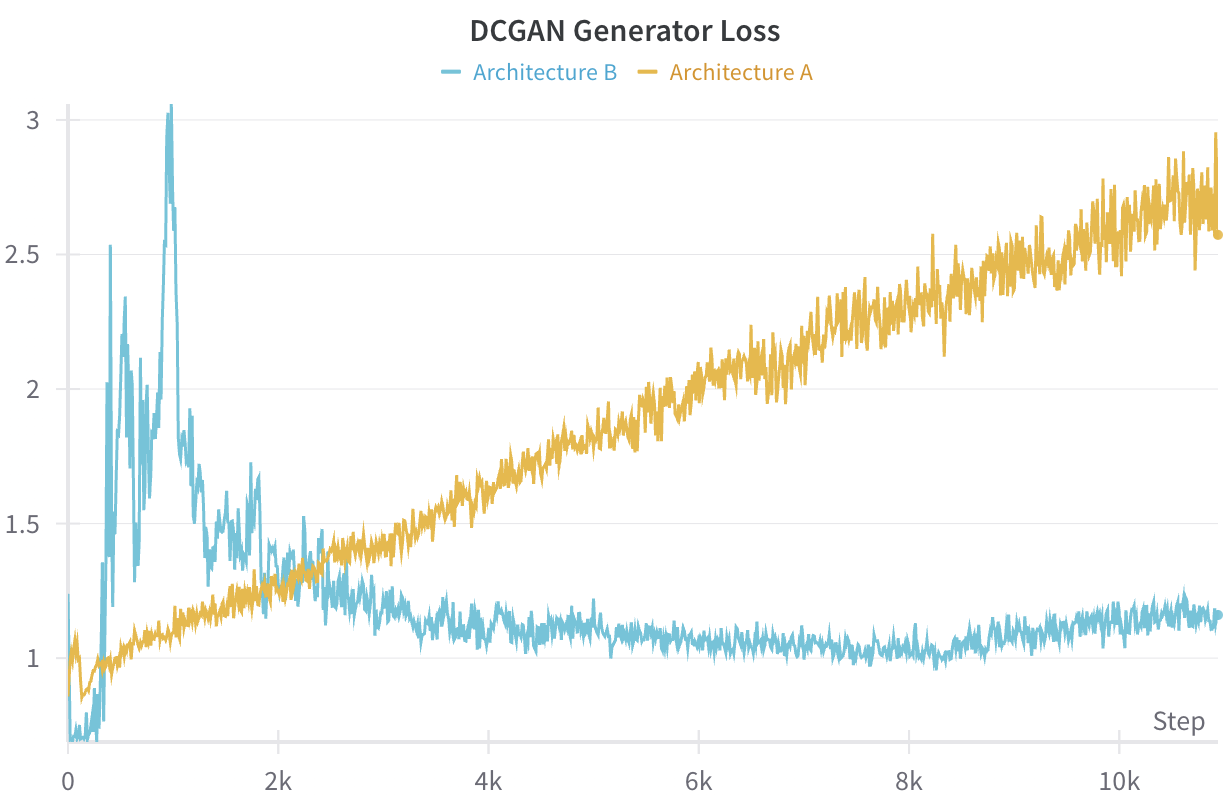
\includegraphics[width=\textwidth]{../src/dc_gen_loss.png}
        \label{fig:image1}
    \end{minipage}
    \hfill
    \begin{minipage}[b]{0.45\textwidth}
        \centering
        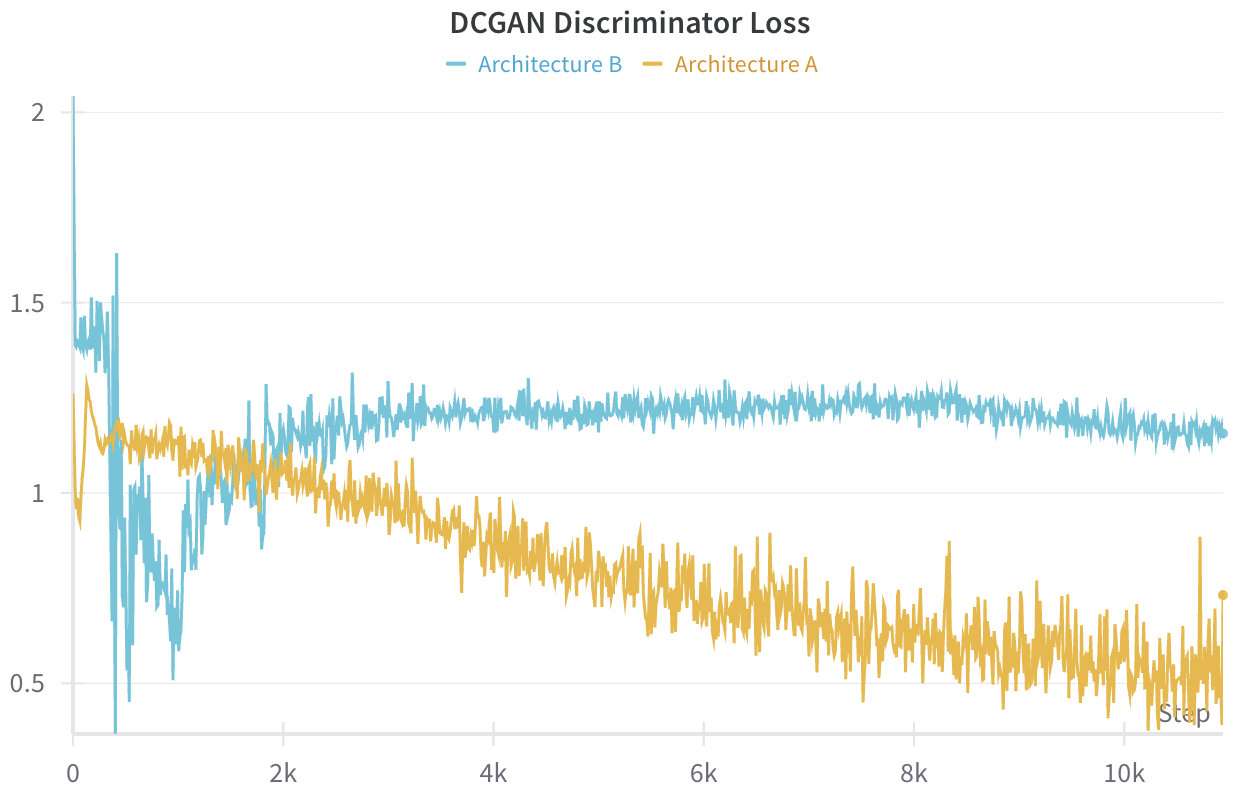
\includegraphics[width=\textwidth]{../src/dc_discrim_loss.png}
        \label{fig:image2}
    \end{minipage}
    % Second row
    \begin{minipage}[b]{0.45\textwidth}
        \centering
        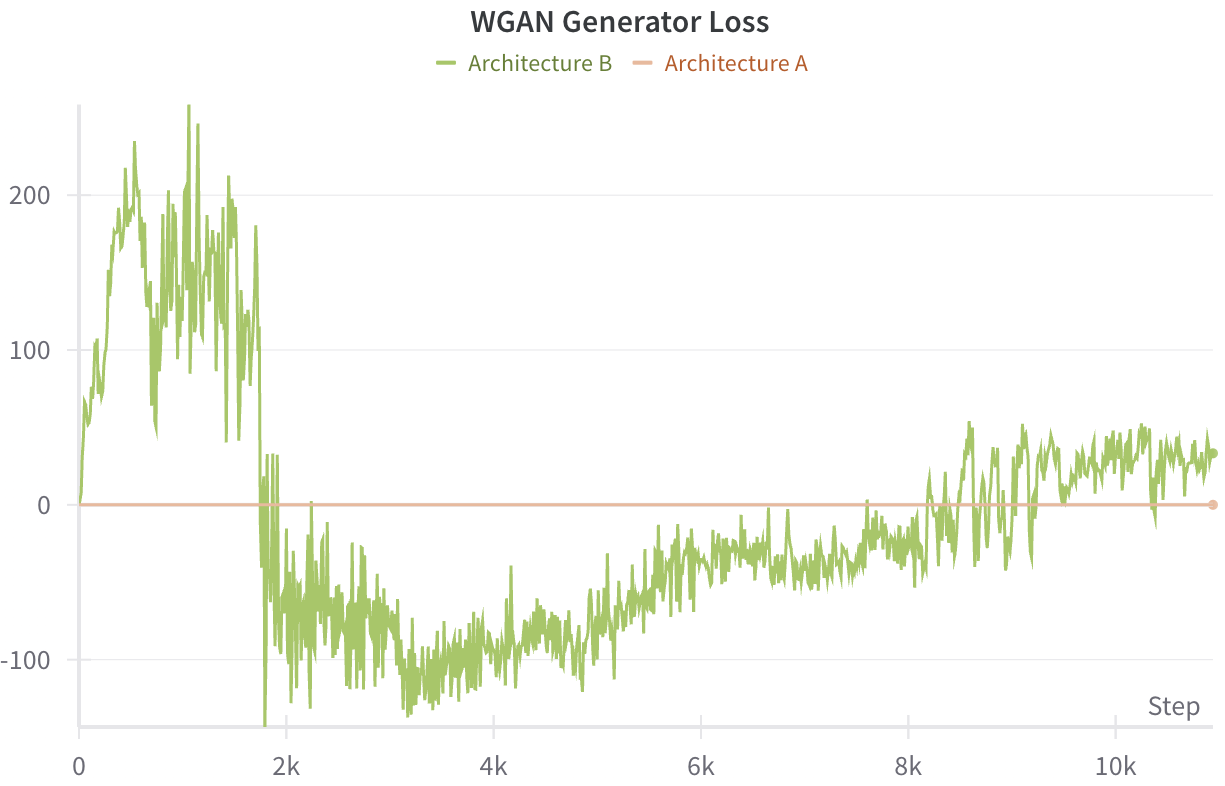
\includegraphics[width=\textwidth]{../src/wgan_gen_loss.png}
        \label{fig:image3}
    \end{minipage}
    \hfill
    \begin{minipage}[b]{0.45\textwidth}
        \centering
        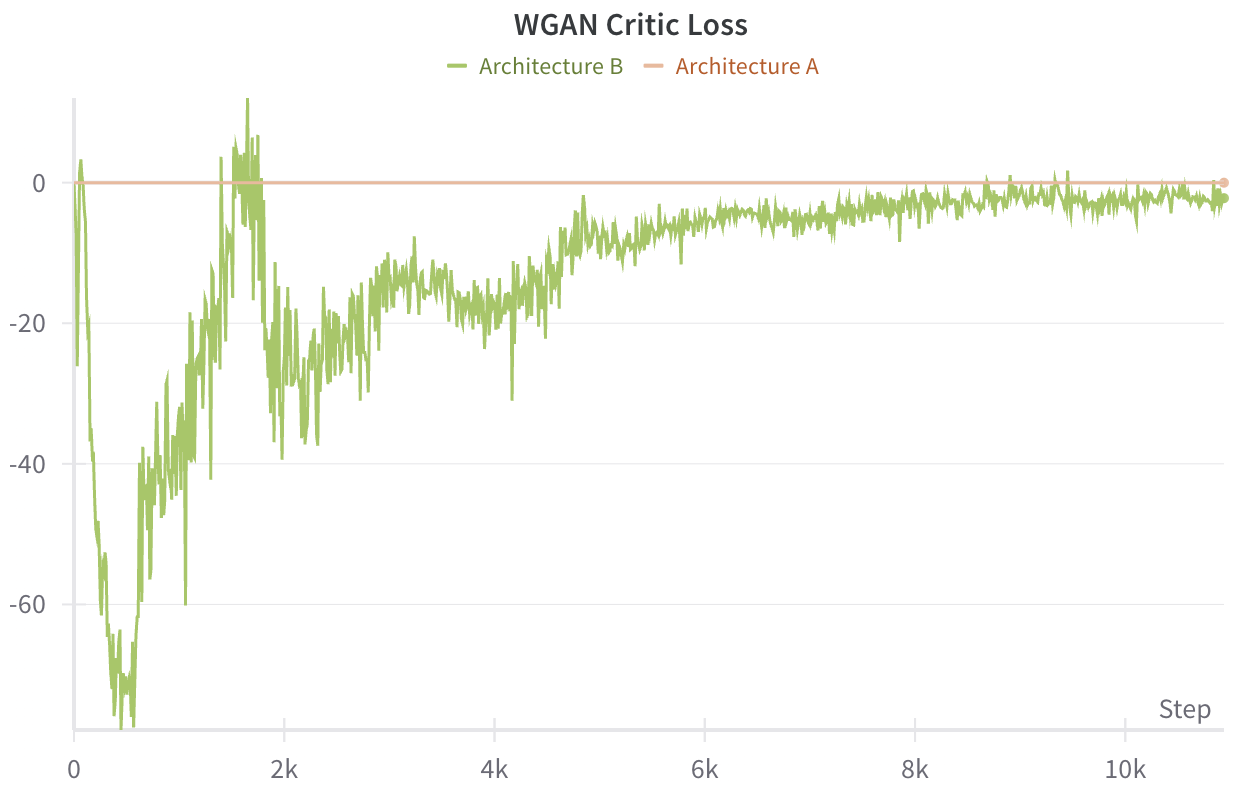
\includegraphics[width=\textwidth]{../src/wgan_crit_loss.png}
        \label{fig:image4}
    \end{minipage}

    % Third row
    \begin{minipage}[b]{0.45\textwidth}
        \centering
        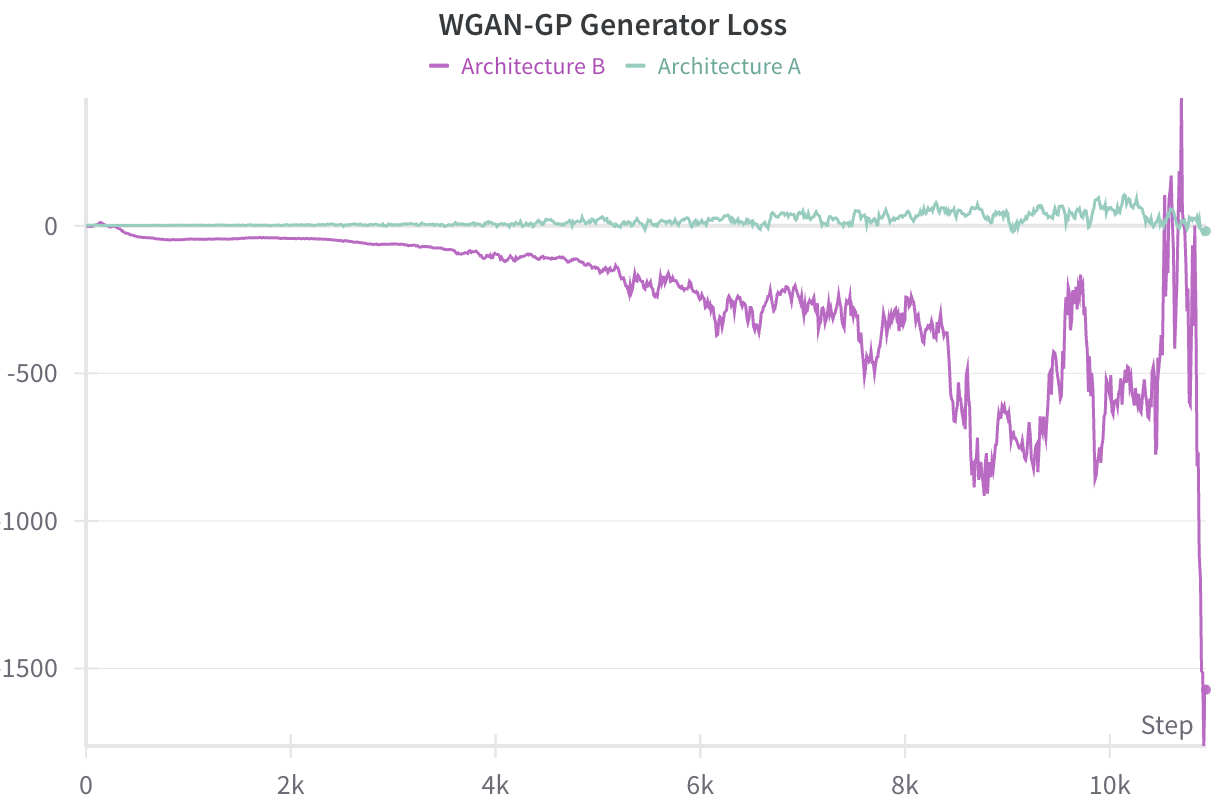
\includegraphics[width=\textwidth]{../src/gp_gen_loss.png}
        \label{fig:image5}
    \end{minipage}
    \hfill
    \begin{minipage}[b]{0.45\textwidth}
        \centering
        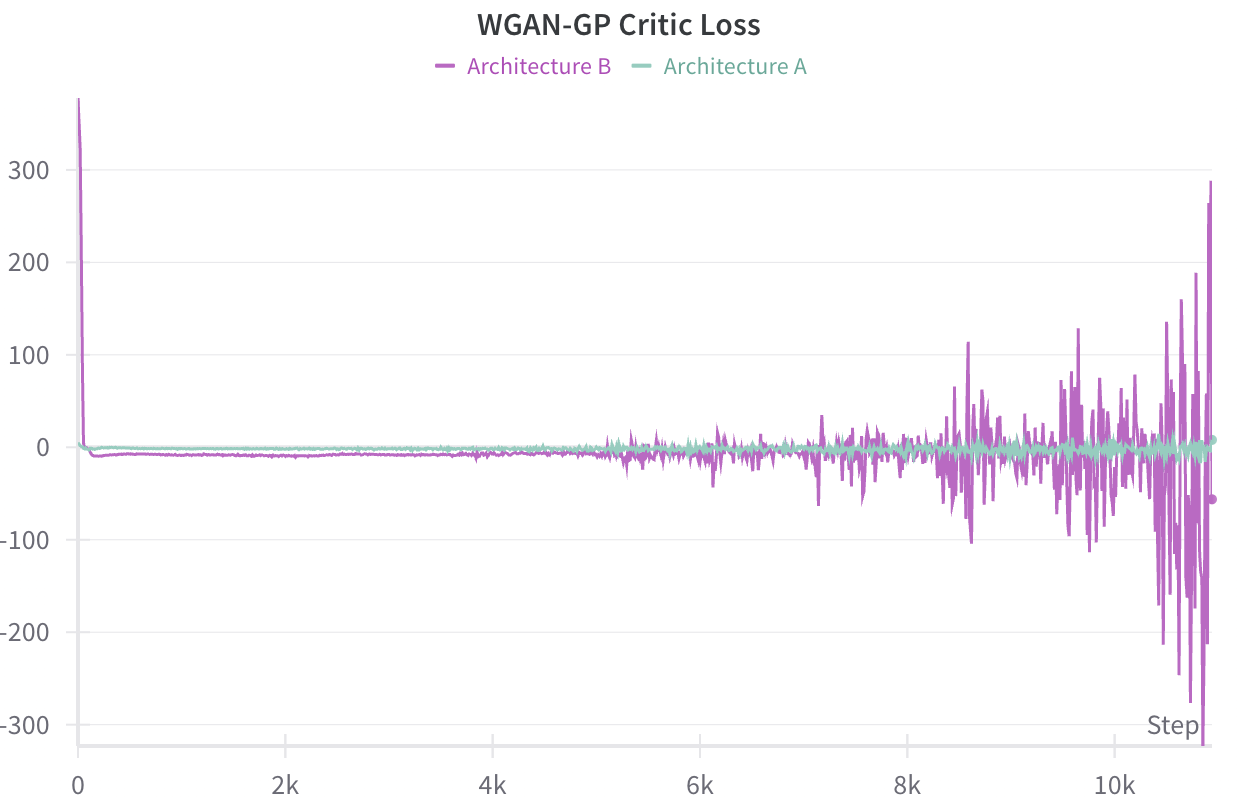
\includegraphics[width=\textwidth]{../src/gp_crit_loss.png}
        \label{fig:image6}
    \end{minipage}

\end{figure}



\begin{figure}[ht]
    \centering
    % First row
    \caption{Zoom-In: Loss Curve for WGAN and WGAN-GP Architecture A}
    \begin{minipage}[b]{0.45\textwidth}
        \centering
        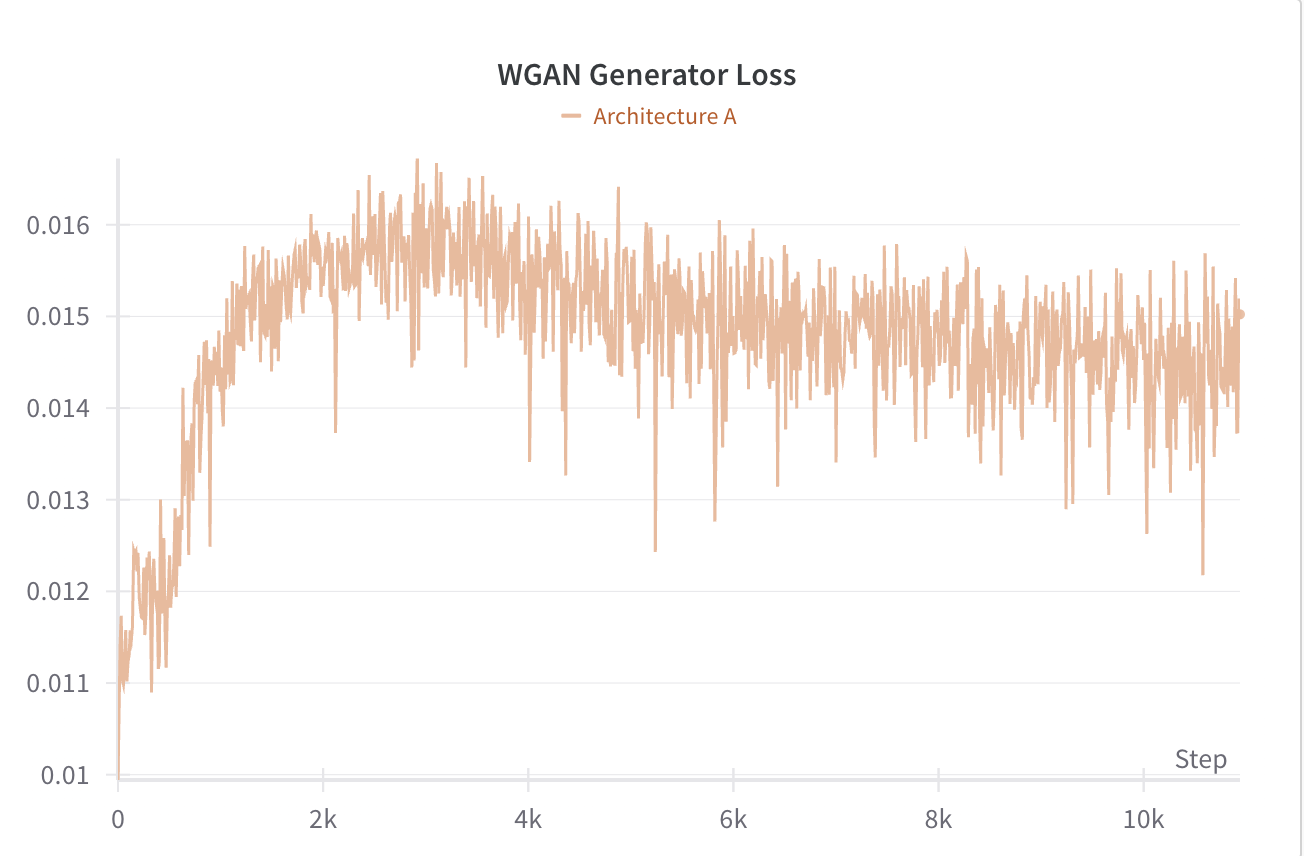
\includegraphics[width=\textwidth]{../src/wgan_zoom_in_gen.png}
        \label{fig:image1}
    \end{minipage}
    \hfill
    \begin{minipage}[b]{0.45\textwidth}
        \centering
        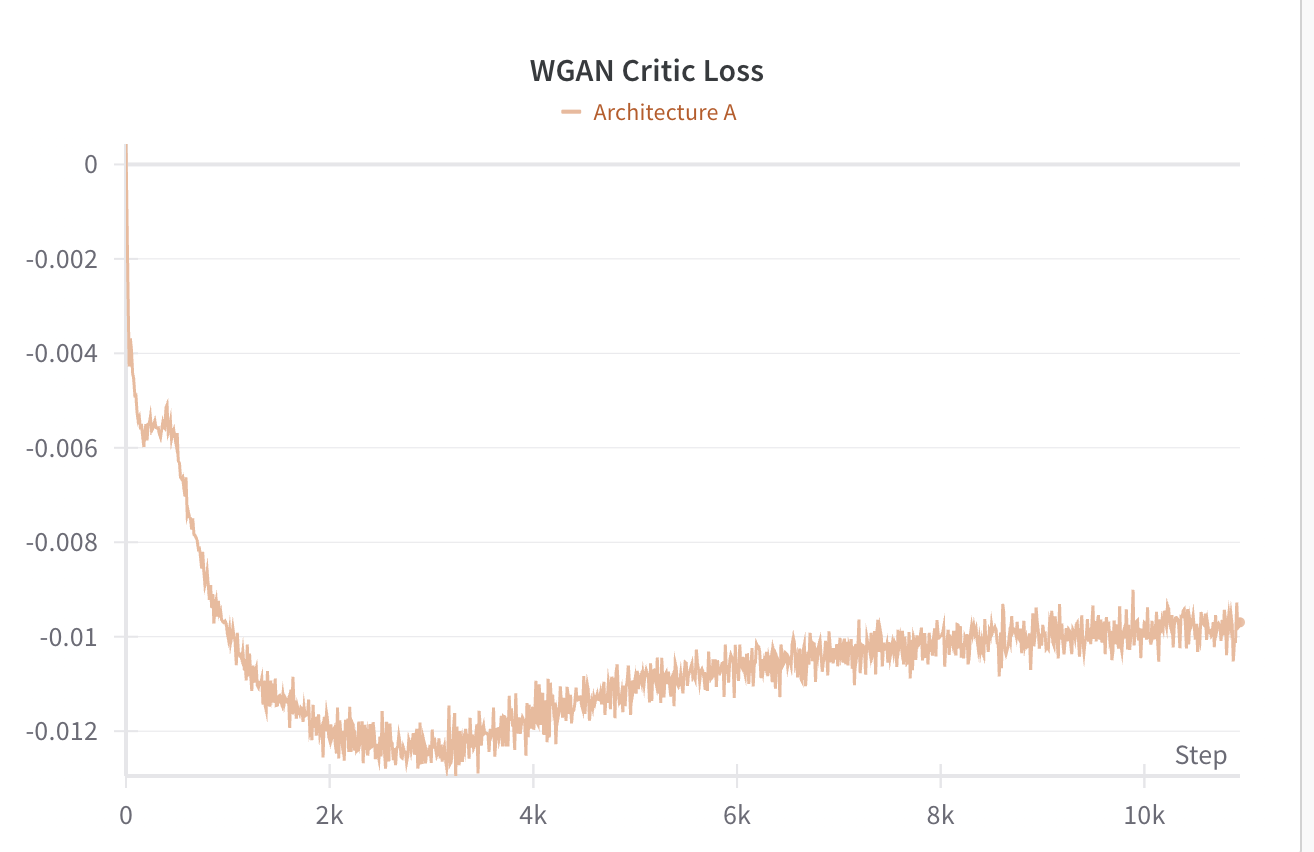
\includegraphics[width=\textwidth]{../src/wgan_zoom_in_crit.png}
        \label{fig:image2}
    \end{minipage}
    % Second row
    % \caption{Zoom-In: Loss Curve for WGAN and WGAN-GP Architecture A}
    \begin{minipage}[b]{0.45\textwidth}
        \centering
        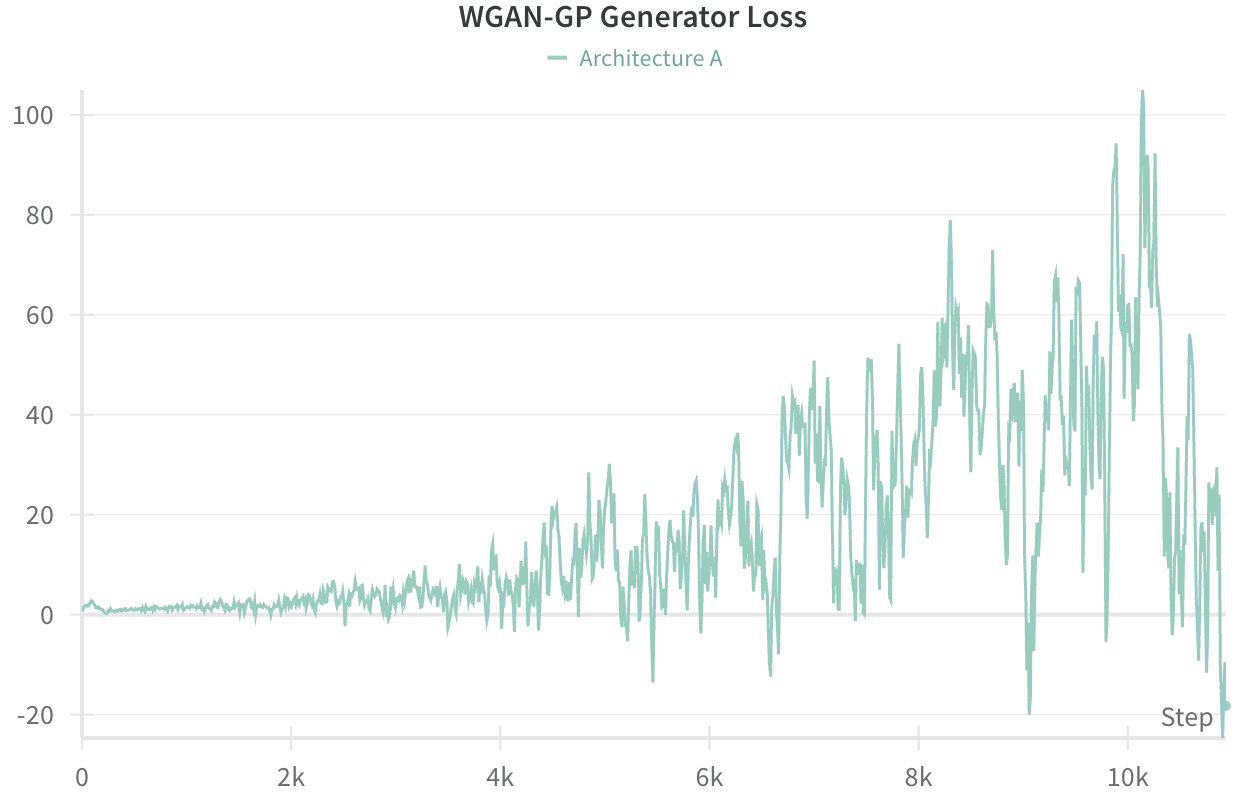
\includegraphics[width=\textwidth]{../src/gp_zoom_in_gen.png}
        \label{fig:image1}
    \end{minipage}
    \hfill
    \begin{minipage}[b]{0.45\textwidth}
        \centering
        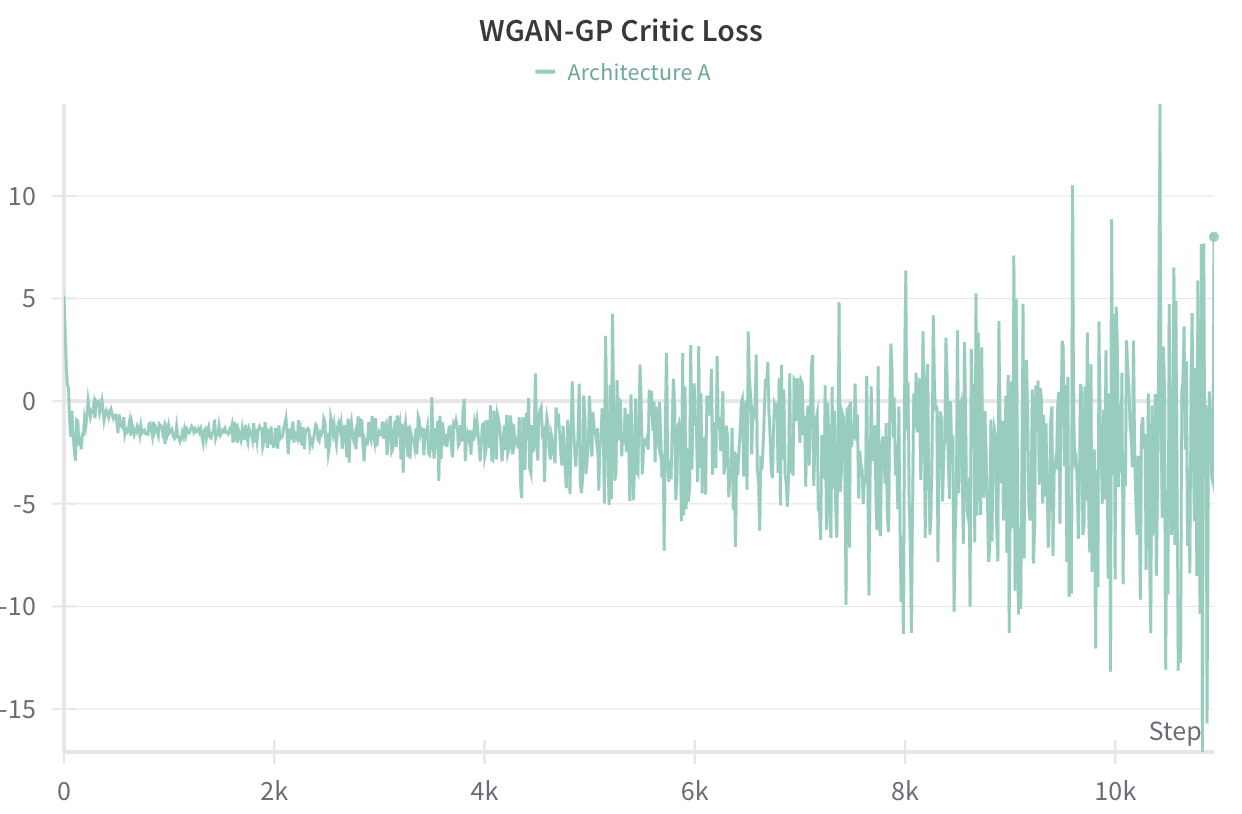
\includegraphics[width=\textwidth]{../src/gp_zoom_in_crit.png}
        \label{fig:image2}
    \end{minipage}
\end{figure}

\end{document}